\usetikzlibrary{decorations.pathreplacing}
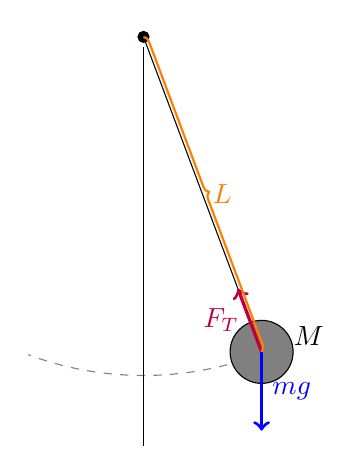
\begin{tikzpicture}

\draw (0,2.5) node (v2) {} -- (1.5,-1.5) node (v1) {};
\draw [fill=gray] (v1) circle (0.4);
\draw [dashed, gray](1.464,-1.5366) arc (-69.6001:-110.4:4.2);
\draw [fill] (v2) circle (0.07);
\draw [ultra thin](v2) -- (0,-2.7);
\draw [very thick, ->, purple](v1.center) -- (1.2,-0.7)node [midway, left]{$F_T$};
\draw [very thick, ->, blue](v1.center) -- (1.5,-2.5)node [midway, right]{$mg$};

\draw [decorate, decoration=brace, draw=orange, thick] (v2.center) -- (v1.center) node [midway, right, orange]{$L$};
\node at (2.1,-1.3) {$M$};
\end{tikzpicture}